\chapter{PLink Collectives: Towards Cloud-aware Collectives with Rank Reordering}
We now shift our focus from building efficient parameter servers to another popular paradigm: collectives, used in popular training frameworks such as Caffe2 and Pytorch, where there is no longer role of servers and workers. We also address the need for specialization on alternative interconnects other than a fat tree topology in the datacenter, e.g., with a torus ring in Google TPU pods, because in these highly specialized environments, our optimizations highlighted earlier may not be sufficient. 

%Our experimental application of \cmpi on \textit{allreduce} operations in public clouds results in a speedup of up to 3.7x in multiple microbenchmarks and 1.3x in real-world workloads of distributed training of deep neural networks and gradient boosted decision trees using state-of-the-art frameworks.

\section{Unoptimal use of Collectives Today}
\mpi algorithms work by decomposing a compound operation into a series of point to point operations between two ranks of nodes according to a predefined communication schedule. Generally, the ranks of nodes are assigned from a list of IP addresses, which assumes no particular order. Since the \mpi algorithms dictate communication on top of the rank abstraction, the outcome does not rely on a specific mapping of IP address to rank.

\begin{figure}[h!]
	\centering
	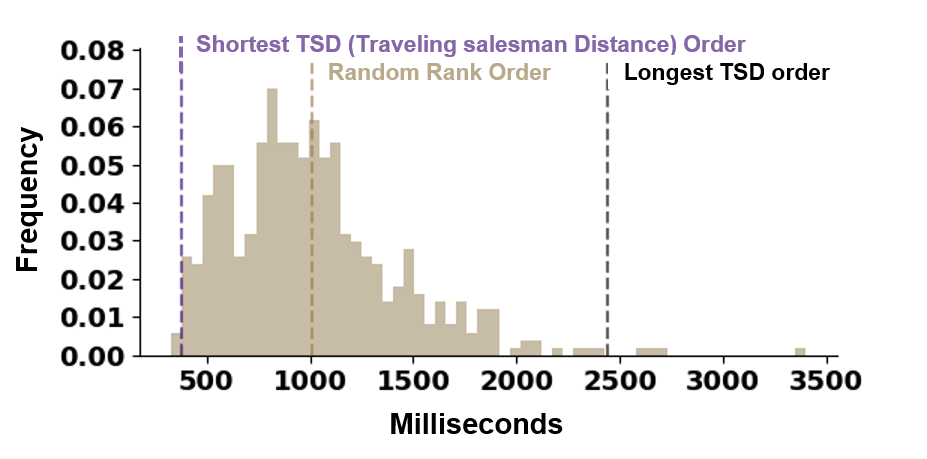
\includegraphics[width=.5\linewidth, trim=8 3 14 14,clip]{Figures/azringperformance.png}
	\caption{Performance distribution of \textit{allreduce} task of 100MB data with ring algorithm varies widely with 500 random rank orders on \azure.}
	\label{fig:azringperformance}
\end{figure}

However, such straightforward use of \mpi with a random mapping from VM node to rank in a cloud context can lead to subpar performance. For example, consider an \textit{allreduce} operation using a \textit{ring} algorithm, where VMs passes data through a virtual ring. In this case, are different ways of forming ring exhibit the same performance? The answer is most likely no, as the ring that corresponds to shorter traveling salesman distance will likely perform better~(Figure~\ref{fig:azringperformance}). On the other hand, not all ways of forming rings achieves the same cost, because the \textit{point to point communication cost is different across VMs~(Figure~\ref{fig:dcnetworkcondition}), i.e., there is locality in the datacenter network itself}, due to the hierarchical structure of the datacenter network, and the dynamic nature of traffic from other tenants. In fact, this observation holds true for many other \mpi algorithms, and it hints that \textit{the VM to rank mapping that extracts most locality from the physical network leads to best performance}. 

We present \cmpi (Cloud-aware \mpi), a prototype tool that accelerates \mpi operations by reordering the ranks of participating VMs such that the communication pattern dictated by the selected \mpi operation best exploits the locality in the network. \cmpi is non-intrusive, requires no code changes nor rebuild of existing application, and runs without support from cloud providers. 

\section{Design and Implementation}
Our work focuses on discovering a permutation of the IP list that exploits the network locality for efficient communication, in a completely transparent way, by minimizing the performance model of a given \mpi algorithm materialized with measured point to point VM communication cost. To do so, we need to (1) efficiently identify the underlying network bandwidth/latency constraints (or collectively, locality); (2) accurately build cost model for the \mpi operation at hand; (3) effectively approximate the minimum of these complex cost functions.

We now describe \cmpi, a tool that takes in a list of VM nodes and a target \collectives algorithm, accurately and efficiently probes their pairwise distance, and uses that information to construct a rank order of VMs that attempts to minimize the total cost of communication.

\subsection{Cost Model for \collectives Algorithms}
\cmpi builds cost model $\mathbb{C}_\mathbb{O}$ for each \collectives algorithm $\mathbb{O}$ parameterized with the number of participating nodes $N$ and size $S$. This section details the cost models for popular algorithms. We use $c_{i,j}(S)$ to refer to the cost for transferring $S$ amount of data from node $i$ to $j$. We further define $MAX_{i=0}^{j}(f(i)) = MAX(f(0),...,f(j))$. We assume $N$ a power of 2 to simplify explanation, and allow arbitrary rank $r$ to alias to canonical rank $(r + N) \text{ mod } N$.
 
\noindent\textbf{Ring}. The cost model of the ring algorithm is the sum of the cost of each hop when traversing the ring: 

$$\mathbb{C}_{r}(N, c, S) = \sum_{i=0}^{N-1} c_{i,i-1}(S)$$

\noindent\textbf{Having Doubling}. Cost of halving doubling is sum of costs for each round of communication, which in turn is the maximum cost of all communications in that round. 

$$\mathbb{C}_{hd}(N, c, S) = \sum_{i=0}^{log_2N-1}MAX_{j=0}^{\frac{N}{2}-1}c_{j,j+2^i}(\frac{S}{2^{i+1}}) $$

\noindent\textbf{Tree}. Cost of running tree algorithm depends on the number of trees and how trees are constructed. The total cost is the maximum cost of all trees, which is in turn determined by the maximum cost of each subtree. We provide a cost model for a popular variant of tree algorithm: double binary tree as used in~\cite{nccl}.
$$\mathbb{C}_{dbt}(N, c, S) = T(0,N-1,S)$$
where $T(i,j,S)$ is expressed recursively: 
\begin{align*}
 T(i,j,S) = 
 \left\lbrace
\begin{array}{l@{}l}
0 \textbf{ if $i \ge j$}\\
MAX(c_{\frac{i+j}{2}, \frac{3i+j}{2}-1}(\frac{S}{2}) + T(i, \frac{i+j}{2}-1), \\
c_{\frac{i+j}{2}, \frac{i+3j}{2}+1}(\frac{S}{2}) + T(\frac{i+j}{2}+1, j)) \textbf{ otherwise}
\end{array}
\right.
\end{align*}
Similarly a mirrored tree is built by decrementing each node's rank in the tree without changing the tree structure.

\noindent\textbf{BCube}. Cost of running tree algorithm is similar to halving doubling, except in each round, each node communicates with $B-1$ peers, instead of 1.

$$\mathbb{C}_{b}(N, c, S, B) = \sum_{i=0}^{log_BN-1}MAX_{j=0}^{\frac{N}{B}-1}MAX_{k=1}^{B}c_{j,j+kB^i}(\frac{S}{B^{i+1}}) $$

\subsection{Probing for Pairwise Distance}
We now need to determine values for $c_{i,j}(S)$ with end-to-end measurements. We first consider commonly used, simple linear model: $c_{i,j} = LAT_{i,j} + \frac{S}{BW_{i,j,S}}$ where $LAT_{i,j}$ being the one-direction latency from $i$ to $j$, and $BW_{i,j,S}$ the bandwidth achieved with data size of $S$. There are immediate challenges of deriving $BW_{i,j}$ correctly: first, $BW_{i,j,S}$ varies depending on the size of packet size $S$ being transferred: e.g., on a 10Gbps link it is unlikely to saturate full bandwidth while sending packet of a few bytes. Figure~\ref{fig:tcpchartacteristics} (left) shows the how bandwidth varies with the size of the buffer in a point to point \textit{iperf} (TCP, using DCTCP) test on two 30Gbps D64 nodes on \azure. It would be cumbersome to create such profile for each pair of VMs; second, even if a profile like this is constructed, it may still fall short in case where multiple streams are competing for bandwidth: the streams do not share the bandwidth equally, but rather, one stream can consistently outperform the other in a long time trace, as shown in Figure~\ref{fig:tcpchartacteristics} (right) with 3 D64 nodes on \azure, when both of them can achieve similar throughput when run individually. It seems intractable to derive an accurate $BW$ given $S$ and a set of competing streams. Third, many \collectives algorithms operate in chunked mode, allowing overlapping of sending (of processed elements) and receiving (of unprocessed elements), and the simple model does not capture this in the first place.

It would be both beneficial and interesting to accurately model throughput behavior in a multi-stream environment~\cite{data-center-tcp-dctcp,tcphsfairness,10.1007/978-3-540-72606-7_86,ha2008cubic}, but that subject is worthy of its own topic. Instead, we compromise by dropping the bandwidth component in the model, leaving only the latency component. The rationale behind this stems from the well-known theoretical TCP bandwidth model of $BW=O(\frac{MSS}{RTT\sqrt{p}})$ ~\cite{mathis1997macroscopic} given constant drop rate $p$ and window $MSS$. The fact that higher latency induces lower bandwidth in TCP streams lets us approximate costs by only probing for latency.

Our tool for distance probing used in \cmpi is similar to that used in \plink.


\begin{figure}[t!]
	\centering
	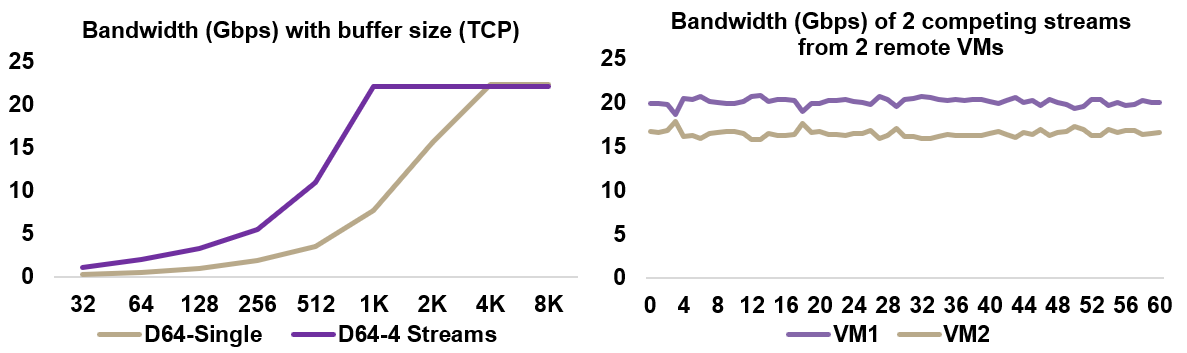
\includegraphics[width=.6\linewidth]{Figures/tcpchartacteristics.png}
	\caption{Left: TCP throughput depends on the buffer size, and number of concurrent streams. Right: while TCP is designed to be fair, an empirical 60s tracing in cloud shows the two streams connecting to the same VM from two other remote VMs do not share the bandwidth equally.}
	\label{fig:tcpchartacteristics}
\end{figure}



\subsection{Minimizing Cost Model}
We now parameterize the cost model with probed $c$. To derive a rank ordering that minimizes $\mathbb{C_O}$, we perform the following transformation: let variables set $\mathbb{R}$ defined as $r_i, i \in [0,N-1]$ be a permutation of $[0,N-1]$ to be solved, and we replace each $c_{i,j}$ with $c_{r_i,r_j}$. We can then establish a bijection from the original rank ordering to the desired order $r_i \leftrightarrow i$ once $r_i$s are solved. We flatten $c_{i,j} \leftrightarrow c'_{iN + j}$ to use theory of arrays to allow direct solving with conventional optimizing SMT solvers such as Z3~\cite{de2008z3,ORToolsG24:online}. 

Unfortunately, we find solvers to be highly inefficient, perhaps due to the non-convex, non-linear nature of the objective function and a large search space ($N!$). Instead, we take a two-stage process. The first step employs a range of stochastic search techniques such as simulated annealing~\cite{simanneal}, with a few standard heuristics (e.g., permuting a random sub-array, permuting random pairs) for obtaining neighboring states and a timeout. When the search returns with an initial result $C_0$, we generate an additional SMT constraint $\mathbb{C_O} < C_0$ to better guide pruning for solvers. We let the solver continue to run for a few minutes, and we either find a better solution or will use $C_0$ as the final value. The end-product of this process is a rearranged list of VMs.